\section{Results}
\label{sec:results}

In this section we demonstrate the efficacy of our novel framework by calculating the first known optimal solutions to the following difficult nonlinear sequential decision problems: (i) inverse learning of parameters in a multi-objective navigation domain; (ii) non-convex optimization of vaccination policy parameters in a public health setting; and (iii) exact sensitivity analysis of portfolio transaction models over the full range of model parameters. Furthermore, we show that our framework is scalable in both space and time. We note that while dOp~\parencite{Gao2013} offer strong delta-optimality guarantees, we found in practice that nonlinear solvers such as $ \mathtt{fmincon} $~\parencite{MATLAB_2010} perform comparably well at optimization and are much more efficient, hence we use solver $ \mathtt{fmincon} $ in the experiments.

%%%%%%%%%%%%%%%%%%%%%%%%%%%%%%%%%%%%%%%%%%%%%%%%%%%%%%%%%%%%%%%%%%%%%%%%%%%
%\begin{figure*}[h!]
%    \vspace{-5mm}
%    \begin{center}
%        \begin{tabular}{ccc}
%            \hspace{-4mm} \includegraphics[width=0.35\textwidth]{images/robot_opt}\label{fig:navigation_opt} & \hspace{-7.5mm} \includegraphics[width=0.35\textwidth]{images/sir_opt} & \hspace{-8mm} \includegraphics[width=0.35\textwidth]{images/oe_opt}\\ 
%            (a) & (b)\label{fig:sir_opt} & (c)\label{fig:oe_opt} \\
%            %\multicolumn{3}{c}{}
%        \end{tabular}
%    \end{center}
%%    \vspace{-4mm}
%    \caption{Nonlinear optimization results for: (a) Maximal weight under a sub-optimal movement policy; (b) Optimal vaccination proportion {\footnotesize $ \nu $} for {\footnotesize $ 0.0 \leq \beta \leq 1.0 $}; and (c) Optimal sell proportion $ \theta $ for {\footnotesize $ inventory \in \left(0.0, 1000.0 \right) $}. }
%    \label{fig:xadd}
%    \vspace{-2mm}
%\end{figure*}
%%%%%%%%%%%%%%%%%%%%%%%%%%%%%%%%%%%%%%%%%%%%%%%%%%%%%%%%%%%%%%%%%%%%%%%%%%%

%\begin{figure*}
%    \begin{multicols}{4}
%        \includegraphics[width=\linewidth]{images/robot_opt}\par\caption{caption} 
%        \includegraphics[width=\linewidth]{images/sir_opt}\par \caption{caption}
%        \includegraphics[width=\linewidth]{images/oe_opt}\par \caption{caption}        
%    \end{multicols}
%    \caption{caption here}
%\end{figure*}
%
%\begin{figure*}
%    \begin{multicols}{4}
%        \includegraphics[width=\linewidth]{images/vf_robot}\par\caption{caption} 
%        \includegraphics[width=\linewidth]{images/vf_sir}\par \caption{caption}
%        \includegraphics[width=\linewidth]{images/vf_oe}\par \caption{caption}        
%        \includegraphics[width=\linewidth]{images/vf_oe_deriv}\par \caption{caption}                
%    \end{multicols}
%    \caption{caption here}
%\end{figure*}

{\centering
    \begin{figure*}[ht]
        \begin{tabular}{cccc}
            \begin{subfigure}{0.24\textwidth}\centering\includegraphics[width=1.0\linewidth]{images/vf_robot}\caption{The value function under the optimal policy.}\label{fig:navigation_vf}\end{subfigure}&
            \begin{subfigure}{0.24\textwidth}\centering\includegraphics[width=1.0\linewidth]{images/vf_sir}\caption{Optimal Value Function for varying {\footnotesize $ \beta $} and {\footnotesize $ \nu $}.}\label{fig:sir_vf}\end{subfigure}&
            \begin{subfigure}{0.24\textwidth}\centering\includegraphics[width=1.0\linewidth]{images/vf_oe}\caption{Optimal Value Function for varying {\footnotesize $ \theta $} and {\footnotesize $ inventory $}.}\label{fig:oe_vf}\end{subfigure}&
            \begin{subfigure}{0.24\textwidth}\centering\includegraphics[width=1.0\linewidth]{images/vf_oe_deriv}\caption{Optimal Value Function for varying {\footnotesize $\nabla \theta $} and {\footnotesize $ inventory $}.}\label{fig:oe_vf_deriv}\end{subfigure}\\            
        \end{tabular}
        \caption{Value functions.}
        \label{tab:vf_Results}
    \end{figure*}
}

{\centering
    \begin{figure*}[ht]
        \begin{tabular}{ccc}
            \begin{subfigure}{0.3\textwidth}\centering\includegraphics[scale=0.25]{images/robot_opt}\caption{Maximal weight under a sub-optimal movement policy}\label{fig:navigation_opt}\end{subfigure}&
            \begin{subfigure}{0.3\textwidth}\centering\includegraphics[scale=0.25]{images/sir_opt}\caption{Optimal vaccination proportion {\footnotesize $ \nu $} for {\footnotesize $ 0.0 \leq \beta \leq 1.0 $}}\label{fig:sir_opt}\end{subfigure}&
            \begin{subfigure}{0.3\textwidth}\centering\includegraphics[scale=0.25]{images/oe_opt}\caption{Optimal sell proportion $ \theta $ for {\footnotesize $ inventory \in \left(0.0, 1000.0 \right) $}}\label{fig:oe_opt}\end{subfigure}\\
        \end{tabular}
        \caption{Nonlinear optimization results.}
        \label{tab:opt_results}
    \end{figure*}
}

\subsection{Multi-objective Navigation}
\label{sec:results_navigation}

In this domain we consider an autonomous vehicle moving in one dimension towards a goal region. At each stage the vehicle faces a trade-off between reaching the goal region and incurring a movement cost. The domain is specified as follows: {\footnotesize $ \State = \left\langle loc \right\rangle$}, where $ loc $ is the location of the vehicle. {\footnotesize $ \Action \in \left\lbrace 0.0, 5.0 \right\rbrace $} is the amount by which vehicle moves relative to its current location. {\footnotesize $ \Transition\left( loc' | loc, a \right) = \delta \left[ loc' - (loc + a) \right] $}, where {\footnotesize $ a \in \Action $}. {\footnotesize $ \Reward\left(\vec{w}, loc, a \right) = w_1 \cdot \Reward_{\mathtt{region}} + w_2 \cdot \Reward_{\mathtt{move}} $} where,
{\footnotesize 
    \abovedisplayskip=10pt
    \belowdisplayskip=0pt
    \renewcommand{\arraystretch}{1.5}
    \begin{tabular}{ll}    
        $ \Reward_{\mathtt{region}}(loc') = $ &  $ $ \\
        \qquad $ \begin{cases}
        (loc' \geq 10.0 ) : & loc' \\
        \text{otherwise} : & 0.0 \\
        \end{cases} $ & $ $\\
        $ \Reward_{\mathtt{move}}(\cdot) = -cost_{\mathtt{move}} \cdot (loc' - loc)$ & $ $ \\                        
    \end{tabular}
} 

Figure~\ref{fig:navigation_vf} and Figure~\ref{fig:navigation_opt} show the {\footnotesize$ \Horizon = 15 $} value function under the optimal and a sub-optimal policy, respectively. We define the sub-optimal policy as $ \pi(0 < loc < 10) = 5.0,  \pi(loc < 0 \,\mathrm{or}\, loc > 10) = 0.0$. The optimal value function reveals that the vehicle is willing to incur the movement cost in order to reach the reward region for low values of {\footnotesize $ w_2 $}, but not otherwise. Figure~\ref{fig:navigation_opt} shows the maximal {\footnotesize $ w_2 $} associated with the actions executed by the vehicle in each state. We notice that in regions where the vehicle does not move, {\footnotesize $ w_2 $} was at its maximum i.e. the movement cost was too great for the vehicle to move. However, in the region where the vehicle did move, the {\footnotesize $ w_2 $} increases as the location approaches the goal region, indicating that the vehicle is willing to incur a greater movement cost to reach the goal region.

%%------------------------------------------------------------------------------
%% Figure
%\begin{figure}[h!]
%    \centering
%    \begin{subfigure}{0.4\textwidth}
%        \includegraphics[width=0.8\linewidth, height=0.5\linewidth]{images/vf_robot}
%        \caption{The value function under the optimal policy.}
%            \label{fig:navigation_vf}
%    \end{subfigure}
%%    \begin{subfigure}{0.4\textwidth}
%%        \includegraphics[width=0.8\linewidth, height=0.5\linewidth]{images/robot_opt}
%%        \caption{The value function under a sub-optimal policy.}
%%            \label{fig:navigation_opt}
%%    \end{subfigure}
%    \caption{Multi-objective navigation when {\footnotesize $w_1 = 1.0$}, {\footnotesize $ \mathtt{threshold} = 10.0 $} and {\footnotesize$ cost_{\mathtt{move}} = 1.0$.}} 
%    \label{fig:vehicle1d}            
%\end{figure}
%%------------------------------------------------------------------------------

\subsection{Influenza Public Health Policy}
\label{sec:results_influenza}

In this domain we address the optimization of a static parameterized vaccination policy under a model of Influenza epidemiology. The decision maker must balance the cost of vaccination and the burden of disease on the population. The domain is specified as follows: {\footnotesize $ \State = \left\langle s, i, r \right\rangle$}, where $ s $, $ i $, and $ r $ refer to the size of the susceptible, infected and recovered sub-populations, respectively. {\footnotesize $ \Action \in \left\lbrace \pi(\nu) \right\rbrace $} where {\footnotesize $\nu in (0.0, 1.0)$} is the proportion of $ s $ to vaccinate at each stage. The transition function {\footnotesize \Transition} for each state variable in {\footnotesize \State} is given by:
    {\footnotesize 
        \abovedisplayskip=5pt
        \belowdisplayskip=0pt
        \renewcommand{\arraystretch}{1.5}
        \begin{tabular}{ll}
            $ \Transition\left( s' | s, i, r, \nu \right) =$ & $ \delta \left[ s' - (s - \beta \cdot s \cdot i - \nu \cdot s) \right] $ \\
            $ \Transition\left( i' | s, i, r, \nu \right) =$ & $ \delta \left[ i' - (i + \beta \cdot s \cdot i - \lambda \cdot i) \right] $ \\
            $ \Transition\left( r' | s, i, r, \nu \right) =$ & $ \delta \left[ r' - (r + \lambda \cdot i + \nu \cdot s) \right] $ \\            
        \end{tabular}
    }%
   
The reward is specified as {\footnotesize $ \Reward\left(cost_{\mathtt{inf}}, cost_{\mathtt{vaccine}}, s, i, r, \nu \right) = (s \cdot (-cost_{\mathtt{vaccine}} \cdot \nu + (1 - \nu))) - cost_{\mathtt{inf}} \cdot i + r$}. {\footnotesize $ cost_{\mathtt{inf}} $} is the incident cost of infection, akin to a burden of disease, and {\footnotesize $ cost_{\mathtt{vaccine}} $} is the unit cost of vaccination. We assume that the total population is constant and that vaccinated individuals go straight from {\footnotesize $ s $} to {\footnotesize $ r $} without being infected. 

%A schematic diagram of the domain is shown in Figure~\ref{fig:sirs_spec}.
%%------------------------------------------------------------------------------
%% Figure
%\begin{figure}[h!]
%    \centering
%    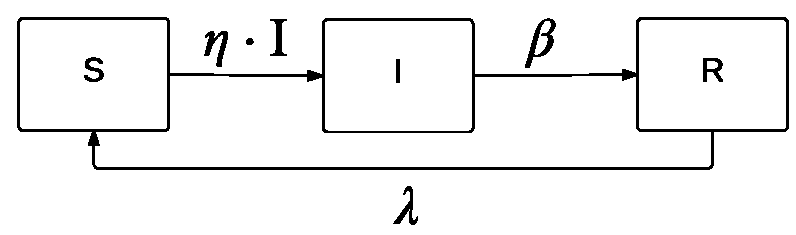
\includegraphics[width=0.5\linewidth, height=0.16\linewidth]{images/sirs}
%    \caption{An S-I-R-S model of Influenza epidemiology.  {\footnotesize $ S $}, {\footnotesize $ I $} and {\footnotesize $ R $} refer to the size of the susceptible, infected and recovered sub-populations, respectively. The infection rate is specified by {\footnotesize $ \beta$}, {\footnotesize $\gamma$} is the rate of recovery and {\footnotesize $\nu$} is the vaccination proportion.}
%    \label{fig:sirs_spec}            
%\end{figure}
%%------------------------------------------------------------------------------

Figures~\ref{fig:sir_vf} and~\ref{fig:sir_opt} show the optimal {\footnotesize $ \Horizon = 7 $} value function and the optimal policy parameter {\footnotesize $ \nu $}, respectively. Figure~\ref{fig:sir_opt} shows that it is optimal to vaccinate the entire susceptible population when {\footnotesize $ \beta > 0.25 $} and none otherwise. This threshold corresponds to the region where the  basic reproductive ratio, {\footnotesize $ R_0 \,(= \beta/\lambda) > 1.0$}. The basic reproductive ratio indicates the average number of secondary cases produced in a typical infection within a completely susceptible population. The optimal policy shows that in this scenario it is worth incurring the vaccination cost to mitigate the costs associated with the burden of disease in an epidemic.

%------------------------------------------------------------------------------
% Figure
%\begin{figure}[h!]
%    \centering
%%    \begin{subfigure}[b]{0.4\textwidth}    
%%        \centering
%%        \includegraphics[width=0.8\linewidth, height=0.5\linewidth]{images/vf_sir}
%%        \caption{Optimal Value Function for varying {\footnotesize $ \beta $} and {\footnotesize $ \nu $}.}
%%        \label{fig:sir_vf}
%%        \vspace{1em}
%%       \end{subfigure}         
%%    \begin{subfigure}[b]{0.4\textwidth}    
%%        \centering
%%        \includegraphics[width=0.8\linewidth, height=0.5\linewidth]{images/sir_opt}
%%        \caption{Optimal {\footnotesize $ \nu $} for {\footnotesize $ 0.0 \leq \beta \leq 1.0 $}. Regions where $ R_0 $, the basic reproductive ratio, is $ < 1 $ and $ > 1 $ are shaded blue and green, respectively. }
%%        \label{fig:sir_opt}
%%     \end{subfigure}         
%    \caption{Influenza Public Health Policy when {\footnotesize $ s = 1000.0, i = 100.0, r = 0.0, \lambda = 0.25 $}, {\footnotesize $ cost_{\mathtt{vaccine}} = 4.0$} and {\footnotesize $ cost_{\mathtt{inf}} = 10.0 $}.}
%    \label{fig:sir}    
%\end{figure}
%------------------------------------------------------------------------------

\subsection{Optimal Execution}
\label{sec:results_oe}

In this domain we examine the sensitivity of an optimal portfolio transaction model to its parameters. Institutional investors often want to transact a number of shares that exceeds available liquidity. In these situations they face a clear trade-off between the market impact of transacting immediately and the volatility of slow execution. The domain is specified as follows {\footnotesize $ \State = \left\langle p, inv \right\rangle$}, where $ p $ is the price of the asset and $ inv $ is the inventory remaining. {\footnotesize $ \Action \in \left\lbrace \pi\left( \theta \right) \right\rbrace$}, where {\footnotesize $ \theta \in \left( 0, 1\right)$} is the proportion of inventory to be sold. The transition function {\footnotesize \Transition} for each state variable in {\footnotesize \State} is given by:
{\footnotesize 
    \abovedisplayskip=5pt
    \belowdisplayskip=0pt
    \renewcommand{\arraystretch}{1.5}
    \begin{tabular}{ll}
        $\Transition\left( p' | p, inv, \pi\left( \theta \right) \right) = $ & $\delta \left[ p' - (p - \kappa \cdot (inv \cdot \pi\left( \theta \right)) + \epsilon) \right] $ \\
        $\Transition\left( inv' | p, inv, \pi\left( \theta \right) \right) = $ & $\delta \left[ inv' - (inv - inv \cdot \pi\left( \theta \right)) \right] $ \\
    \end{tabular}
}%
where {\footnotesize $ \kappa > 0$} is a market-impact parameter and {\footnotesize $ \epsilon $} is a discrete noise parameter. The reward is specified by {\footnotesize $ \Reward\left(p', inv, \pi\left( \theta \right) \right) = p' \cdot inv \cdot \pi\left( \theta \right)$ }.

Figures~\ref{fig:oe_vf} and~\ref{fig:oe_vf_deriv} show the optimal {\footnotesize $ \Horizon = 10 $} value function and its derivative with respect to the parameter {\footnotesize $ \theta  $}, respectively. It is evident that the optimal proportion of shares sold, {\footnotesize $ \theta $}, decreases as inventory increases. When inventory is low, selling a large proportion of shares allows the investor to capture the current price without having too adverse an effect on future prices. This phenomenon is reversed when inventory is high, with the investor selling a lower proportion of shares allows to capture a more stable set of prices by minimising the market impact of their trades on future prices. This insight is confirmed in Figure~\ref{fig:oe_vf_deriv} which shows that the value function is most sensitive to {\footnotesize $ \theta $} when the inventory is high.

%------------------------------------------------------------------------------
% Figure
%\begin{figure}[h!]
%    \centering
%    \begin{subfigure}[b]{0.4\textwidth}    
%        \includegraphics[width=0.8\linewidth, height=0.5\linewidth]{images/vf_oe}
%        \caption{Optimal Value Function for varying {\footnotesize $ \theta $} and {\footnotesize $ inventory $}.}
%        \label{fig:oe_vf}        
%    \end{subfigure}
%    
%    \begin{subfigure}[b]{0.4\textwidth}    
%        \includegraphics[width=0.8\linewidth, height=0.5\linewidth]{images/vf_oe_deriv}
%        \caption{Optimal Value Function for varying {\footnotesize $\nabla \theta $} and {\footnotesize $ inventory $}.}
%        \label{fig:oe_vf_deriv}        
%    \end{subfigure}    
%    
%%    \begin{subfigure}[b]{0.4\textwidth}    
%%        \includegraphics[width=0.8\linewidth, height=0.5\linewidth]{images/oe_opt}
%%        \caption{Optimal $ \theta $ for {\footnotesize $ inventory \in \left(0.0, 1000.0 \right) $}.}
%%        \label{fig:oe_opt}
%%        
%%    \end{subfigure}        
%        \caption{Optimal Execution when {\footnotesize $ \kappa = 0.165 $} and {\footnotesize $ p = 55.0 $}.}
%        \label{fig:oe}    
%\end{figure}
%------------------------------------------------------------------------------

\subsection{Time and Space Complexity}

\begin{figure}[h!]
    \centering
    \begin{subfigure}[b]{0.4\textwidth}    
        \includegraphics[scale=0.25]{images/time_plot}
 %       \caption{Optimal Value Function for varying {\footnotesize $ \theta $} and {\footnotesize $ inventory $}.}
        \label{fig:time_complexity}        
    \end{subfigure}
    
    \begin{subfigure}[b]{0.4\textwidth}    
        \includegraphics[scale=0.25]{images/space_plot}
%        \caption{Optimal Value Function for varying {\footnotesize $\nabla \theta $} and {\footnotesize $ inventory $}.}
        \label{fig:space_complexity}        
    \end{subfigure}    
    \caption{Computational time and space versus {\footnotesize $ \Horizon $} for the Multi-objective navigation domain.}
    \label{fig:time_space_complexity}    
\end{figure}

Figure~\ref{fig:time_space_complexity} shows the relationship between the horizon $ \Horizon $ and the computational time and space for the largest domain. It is clear that our novel framework is capable of calculating scalable solutions in terms of both space and time.

